

%\usepackage{graphicx}
\usepackage{hyperref}
\usepackage{todonotes}

\usepackage{endfloat}
\renewcommand{\efloatseparator}{\mbox{}} % no new page between figures

\usepackage{booktabs} % For formal tables

\settopmatter{printacmref=false} % Removes citation information below abstract
\renewcommand\footnotetextcopyrightpermission[1]{} % removes footnote with conference information in first column
\pagestyle{plain} % removes running headers

\newcommand{\TODO}[1]{\todo[inline]{#1}}



\title{Visualization in Big Data}


\author{Himani Bhatt}
\affiliation{%
  \institution{Indiana University}
  \city{Bloomington} 
  \state{Indiana} 
}
\email{himbhatt@iu.edu}



% The default list of authors is too long for headers}
\renewcommand{\shortauthors}{H. Bhatt}



\begin{abstract}
Data Visualization is the term used for knowing the visual context of data in order to understand its significance. How to unravel the strands of big data to pick out the relevant parts. If we have multiple sources of data how do we know where to look. Data visualization is the solution to all these questions. It helps to convert information into knowledge. Businesses are using big data in order to better understand their customers and to optimize their business processes. In order to find the meaning, tell the story and sharing the story, visualization is needed where data meets design.
\end{abstract}

\keywords{ HID $202$, i$523$, BI(Business Intelligence), DV(Data Visualization).}

\maketitle

\section{Introduction} 

Data visualization is emerging as an important fusion of graphics, scientific visualization, database and human-computer interaction. Data visualization if properly aligned can provide a shorter route for decision making and a way of conveying critical information. For the data visualization to be truly productive, it has to be interactive, meaningful, understandable, user friendly and approachable. The main advantage of data visualization is that it provide insights into complex data sets by communicating their key aspects \cite{Intro01}.Not only insights, it allows users to see different perspective of the data, offers ability to note exceptions in the data, equips users with ability to see influences that would be difficult to find otherwise, helps users finding nuances that are significant \cite{Intro02}. \\

According to Friedman (2008) the ``main goal of data visualization is to communicate information clearly and effectively through graphical means. It doesn't mean that data visualization needs to look boring to be functional or extremely sophisticated to look beautiful. To convey ideas effectively, both aesthetic form and functionality need to go hand in hand, providing insights into a rather sparse and complex data set by communicating its key-aspects in a more intuitive way. Yet designers often fail to achieve a balance between form and function, creating gorgeous data visualizations which fail to serve their main purpose $-$ to communicate information'' \cite{Intro03}.\\

Simple form of data visualization include graphs, pi charts, histograms, scatter plots, and maps. Colors can be used to show correlation, size to show quantity, and orientations used to show trends. Design is used to better communicate varied sorts of information, processes, hierarchy, anamoly and analogy. Tables \ref{table1} and \ref{table2} shows basic type of visualization diagrams with their usage.



\begin{table}[H]

\centering
\begin{adjustbox}{max width=\textwidth}

  \begin{tabular}{ | c | m{3cm} | m{3cm} | }
    \hline
    Data visualization diagrams & Interpretation \\ \hline
    \begin{minipage}{.3\textwidth}
      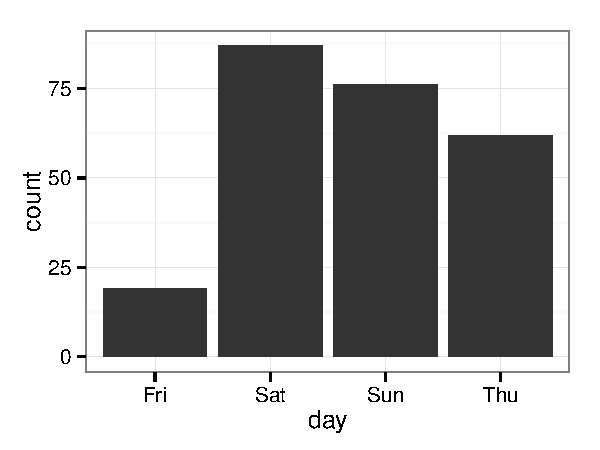
\includegraphics[width=30mm, height=30mm]{images/barchart.pdf}
      \captionof*{figure}{Barchart}
    \end{minipage}
    &
    %\begin{minipage}[t]{3cm}
      Used for comparison of variables against single variable.
          %\end{minipage}
    
    \\ \hline
    
    \hline
  
    \begin{minipage}{.3\textwidth}
      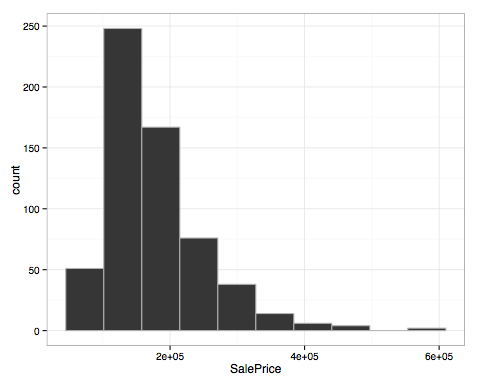
\includegraphics[width=30mm, height=30mm]{images/histogram.png}
      \captionof*{figure}{Histogram}
    \end{minipage}
    &
    %\begin{minipage}[t]{3cm}
      Histogram shows frequency of score occurrences in a continuous data set that has been divided into classes, called bins.
    %\end{minipage}
    
    \\ \hline
    
   \hline
  
    \begin{minipage}{.3\textwidth}
      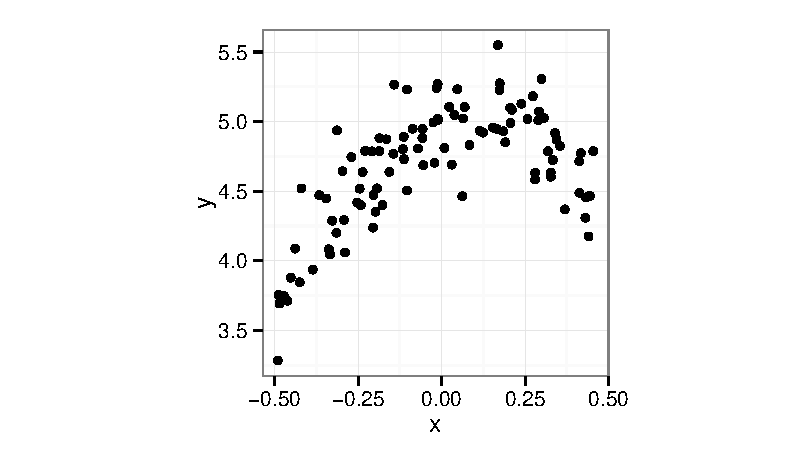
\includegraphics[width=30mm, height=30mm]{images/Scatterplot.pdf}
      \captionof*{figure}{Scatter Plot}
    \end{minipage}
    &
    %\begin{minipage}[t]{3cm}
      Scatter plot is used to show correlation between two variables.
          %\end{minipage}
    
    \\ \hline
    
    \hline
  
    \begin{minipage}{.3\textwidth}
      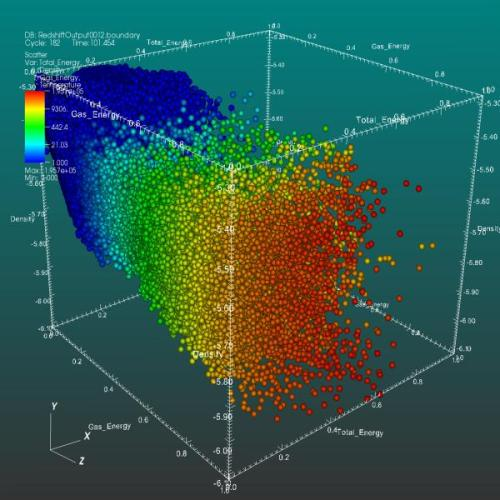
\includegraphics[width=30mm, height=30mm]{images/Scatter_plot3D.jpg}
      \captionof*{figure}{3D Scatter Plot}
    \end{minipage}
    &
    %\begin{minipage}[t]{3cm}
      3D Scatter plot is used to show correlation between three variables.
          %\end{minipage}
    
    \\ \hline
    
    \hline
  
    \begin{minipage}{.3\textwidth}
      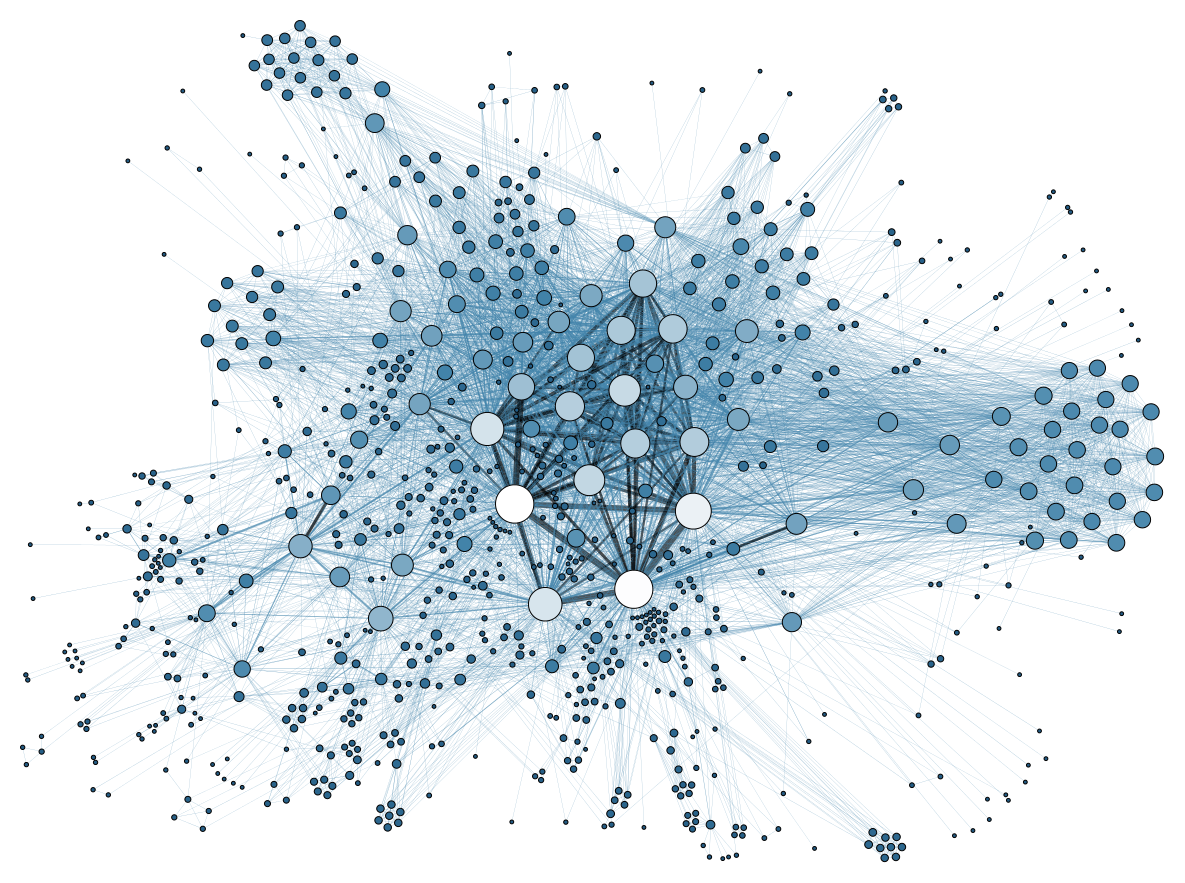
\includegraphics[width=30mm, height=30mm]{images/Network.png}
      \captionof*{figure}{Network}
    \end{minipage}
    &
    %\begin{minipage}[t]{3cm}
      Networks are used for finding clusters in the network, discovering bridges in the network, in determining most influential nodes and in finding outliers who are out of periphery of network.
          %\end{minipage}
    
    \\ \hline
    
  \end{tabular}
  \end{adjustbox}

  \caption{Data visualization diagrams. \cite{Table01}}\label{table1}
\end{table}





\begin{table}[H]
\label{table2}
  \centering
  \begin{adjustbox}{max width=\textwidth}
  \begin{tabular}{ | c | m{3cm} | m{3cm} | }
    \hline
    Data visualization diagrams & Interpretation \\ \hline
    \begin{minipage}{.3\textwidth}
      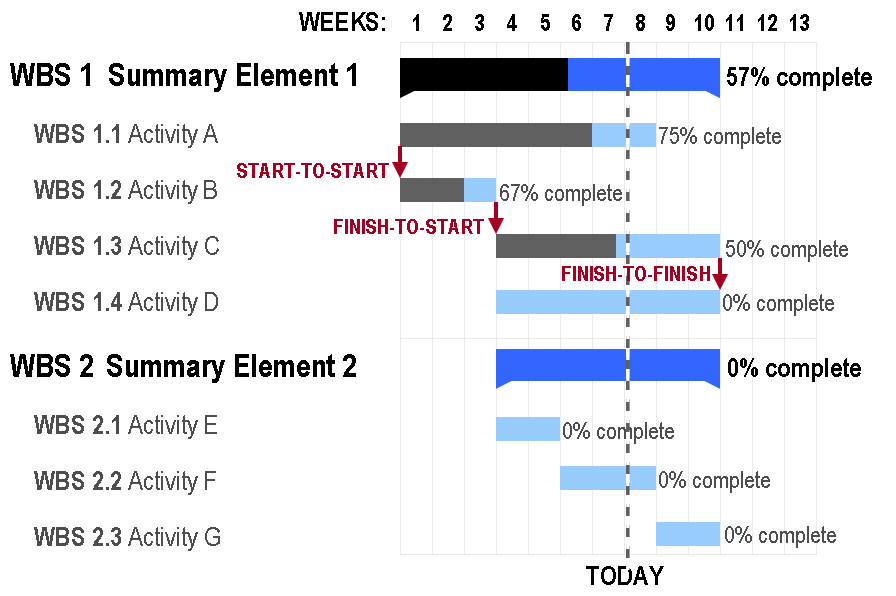
\includegraphics[width=30mm, height=30mm]{images/GanttChart.png}
      \captionof*{figure}{Gantt chart}
    \end{minipage}
    &
    %\begin{minipage}[t]{3cm}
      A Gantt Chart is used as a project management tool to illustrate how the project will run. We can view individual tasks, their duration and the sequencing of these tasks.
          %\end{minipage}
    
    \\ \hline
    
    \hline
  
    \begin{minipage}{.3\textwidth}
      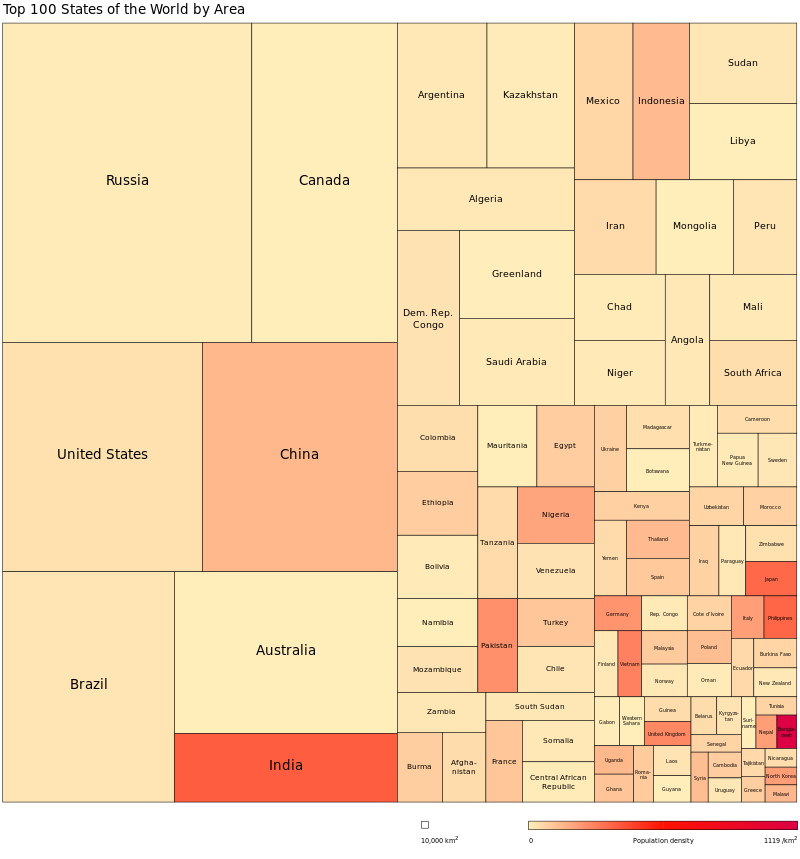
\includegraphics[width=30mm, height=30mm]{images/Treemap.png}
      \captionof*{figure}{Treemap}
    \end{minipage}
    &
    %\begin{minipage}[t]{3cm}
      Treemaps are ideal for displaying large amounts of hierarchically structured (tree-structured) data.
    %\end{minipage}
    
    \\ \hline
    
   \hline
  
    \begin{minipage}{.3\textwidth}
      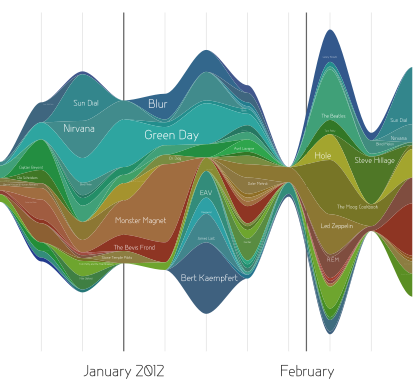
\includegraphics[width=30mm, height=30mm]{images/Streamgraph.png}
      \captionof*{figure}{Stream graph}
    \end{minipage}
    &
    %\begin{minipage}[t]{3cm}
      Stream graph are used to show changes of different categories over time when there are many categories and these categories start and stop at different times. 
    %\end{minipage}
    
    \\ \hline
    
    \hline
  
    \begin{minipage}{.3\textwidth}
      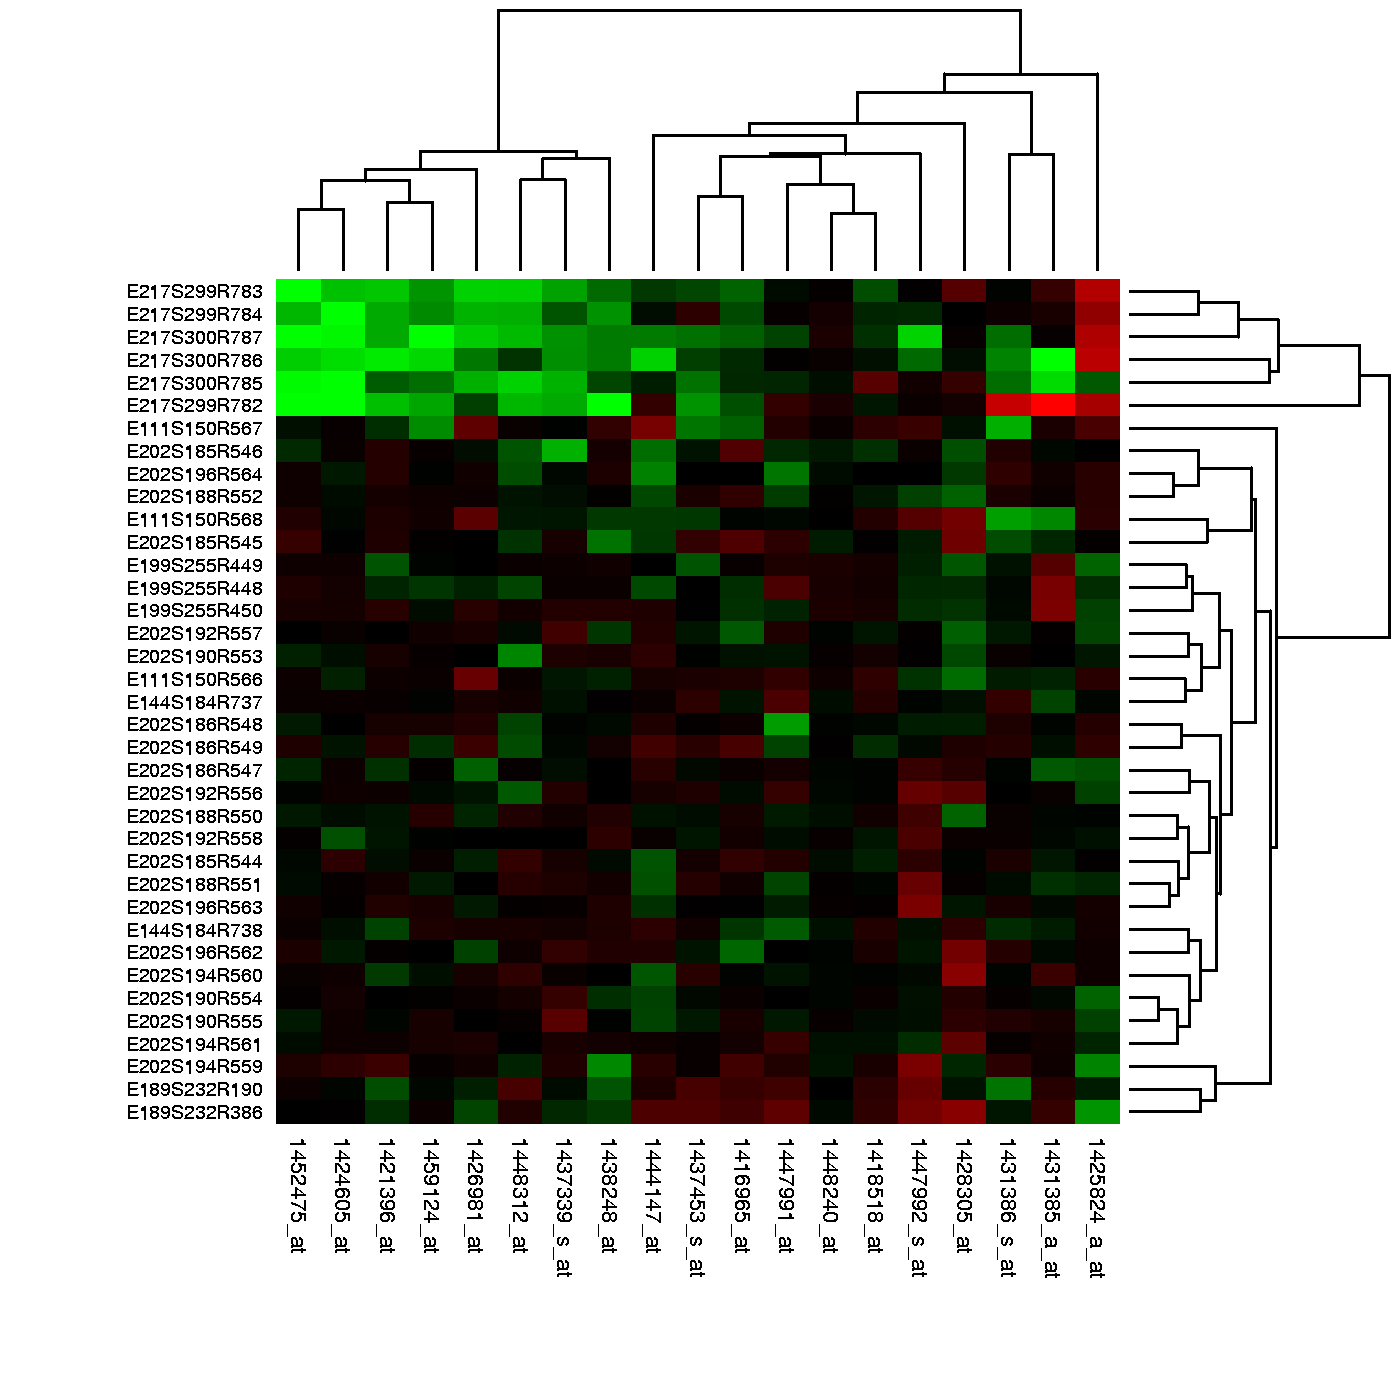
\includegraphics[width=30mm, height=30mm]{images/Heatmap.png}
      \captionof*{figure}{Heatmap}
    \end{minipage}
    &
    %\begin{minipage}[t]{3cm}
      A heat map is a two-dimensional representation of data in which values are represented by colors.
          %\end{minipage}
    
    \\ \hline
    
  
  \end{tabular}
   \end{adjustbox}
  \caption{Data visualization diagrams \cite{Table01}} \label{table2}
\end{table}


\section{Data Visualization tools used by Data Scientists}

There are some excellent open source data visualization tools available that can be used by everyone. All we need to do is to create an account, import the data (in the form of .csv file, Google Sheet etc. and make or pick our own visualizations. Some of them are :

\subsection*{D3.js}

D3.js is a javascript library written by Mike Bostock and is used to create custom visualizations on the web and is open source. It takes advantage of already established web technologies like canvas, SVG. With the advancements in browser technology, it is now possible to render complex visualizations on variety of devices. The setup of machines involves 3 steps - Text Editor, Browser and a Web Server (which will be used to deliver content over the internet). For using D3.js some basic web development skill is required that include knowledge of HTML, CSS, JavaScript and SVG.
D3.js can be used to make visualizations loaded with animations and interactivity. D3 is often used with Crossfilter for quick data manipulation of big data. But since it has tools for manipulating and laying out data in pure javascript, it naturally limits what we can do with javascript in memory (in the browser or in node) \cite{D3}.\\


\subsection*{Google Data Studio}

Data Studio which is an open source tool can be used to create meaningful, shareable visualizations with few clicks. It provides - visual editor to create reports and dashboards, rich library of vizualizations, fully custom design and style controls, reusable templates, dynamic and interactive report controls based on various dimensions available in data, and seamless integration between data analysis and reporting. But Google's Data Studio visualization toolset focuses primarily on connecting up data from Google sources, such as Google Analytics, Google AdWords, Google Sheets, and BigQuery. However it will soon roll out connectors for SQL databases. We can even import big data like facebook data, but the information need to be present in Google Sheet so that it can be pulled into a Google Data Studio \cite{Google}. \\

\subsection*{Microsoft Excel Power Tools}

Latest version of Excel has excellent range of power tools that can be used to analyze and visualize business data. Power Pivot can import and manage millions of data rows for multiple sources. Power Query is another data analysis power tool that can be used for extracting data from a massive range of data sources, to clean and transform that data, that uses the inbuilt JSON parser to build massive data visualizations over Big Data analysis. Power View is an interactive visualization tool used to provide a drag-and-drop interface for rapid model building. It allows updating visualizations on-the-fly and shows data hierarchies allowing to drill down through data. Power Map enables us to plot and visualize data in  three-dimensions. It can plot millions of rows of data across a three-dimensional map, using data taken directly from a table, or using a data model \cite{Excel}.

\subsection*{MATLAB}

The latest version of MATLAB, the numeric computing environment and fourth-generation language, offers new capabilities that allow for the analysis of big data. MATLAB now has built-in MapReduce functionality to allow for analysis of data sets that are too big to fit in memory. Algorithms can be developed on a desktop and then executed on a Hadoop cluster. MATLAB includes all the graphics features required to visualize engineering and scientific data, which includes 2D plots as well as 3D plots. There are functions for plotting topological data, an image data, for 3D volume visualization, for producing animations, and for plotting 3D objects. Sound can also be visualized using MATLAB \cite{MATLAB}.

\subsection*{Mathematica}

Mathematica is used to make high quality automated data visualization with the help of unified architecture. It provides static and dynamic visualization that scales from immediate one-off projects to fully automated industrial-scale production systems. It	offers a powerful suite	of data	analysis and data mining packages, along with a	very rich data visualization framework for its users. Mathematica has its own graphics language,	with which graphics	primitives can be interactively	rendered inside	the	worksheet. This makes Mathematica’s	capability similar to many widely used visualization languages.	Mathematica	provides a plethora	of functions to	combine	these primitives and make them interactive. Along with basic plots, it can be used for time series and scientific visualization, statistic and text visualization, map visualization \cite{Mathematica}.\\

\subsection*{R Programming Language }

R has built in functions and libraries to build visualizations and present data. Charts like scatter plot, histogram, Bar and stack bar chart, box plot, area chart, heat map, correlogram can be made using the library ggplot2. Package heatmaply is used for easily creating interactive cluster heatmaps that can be shared online as a stand-alone HTML file. R package named iplots enhances the interactivity of the graphs. This package provides interactive mosaic plots, bar plots, box plots, parallel plots, scatter plots, and histograms that can be linked together and color brushed. The major advantage of using these is R can be used by anyone and is open source \cite{R}.

\subsection*{Python}

Python comes with a wide range of prebuilt libraries focused on big data processing, visualization, and other data manipulations. Python has multiple libraries that can be practically used for every data visualization need. Matplotlib is a top-notch piece of software which is making Python (with some help of NumPy, SciPy, and Pandas) a cognizant competitor to such scientific tools as MatLab or Mathematica. It can be used to make line plot, scatter plot, bar chart, pie chart, stem plot, contour plot, quiver plots, spectograms. Another library Seaborn is mostly focused on the visualization of statistical models; such visualizations include heat maps, those that summarize the data but still depict the overall distributions. Seaborn is based on Matplotlib and highly dependent on that. Bokeh is another library which is aimed at interactive visualizations and is independent of Matplotlib. Also it makes its presentation via modern browsers in the style of Data-Driven Documents (d3.js). The library Plotly is rather a web-based toolbox for building visualizations, exposing APIs to some programming languages (Python among them). In order to use Plotly, you will need to set up your API key \cite{Python}. 

\section{Commercial Data Visualization Tools}

Visualization solutions are rapidly evolving. Some of the most popular and innovative data visualization tools are : 
\subsection*{Tableau}

Tableau is a data visualization tool created by Tableau Software. Tableau’s data visualization is considered to be more interactive than the ones provided by the general BI solutions. The huge and fast changing datasets used in big data operations, artificial intelligence and machine learning can be handled efficiently because of the integration of tableau with various advance database solutions like Teradata, SAP, Amazon AWS, Hadoop. Tableau offers 5 main products: Tableau Desktop,Tableau Server, Tableau Online, Tableau Reader, Tableau Public \cite{Tableau}.\\

\subsection*{Qlikview}

Qlikview is the business discovery platform. It offers powerful business intelligence, analytics and enterprise reporting capabilities other than the data visualization capabilities. It has a clean and clutter free user interface. It is used with Qliksense, which is responsible for data exploration and discovery. Dynamic calculation is the major innovation in Qlikview. It generate new views of information as the users clicks or taps, and instantly responds with the newly calculated set of data and visualizations \cite{Qlikview}.

\subsection*{Spotfire}

Tibco spotfire is the tool used for business intelligence. It is used by predictive analytics professionals to make imperative decisions. It has a library that helps in transferring analysis that has occurred by hard practices from an expert to business user. It not only increase the speed of decision making but also delivers framework for circulation of analysis applications, that depends on the needs of an association. It also make access to the server based data sources easy, since it has its own analytics servers centrally coped information facilities. It has self configuring visual data analysis environment that helps users to explore, visualize and query data in real time \cite{Spotfire}.

\subsection*{MS BI Stack}

Microsoft BI Stack provides all the tools we need to build, manage and use a BI solution, as part of Microsoft SQL Server, Sharepoint and Office applications. Visual studio 2015 can be used to get business insights on a platform that is designed to work with the data, systems and tools. For the enterprises using Microsoft technologies, Microsoft BI stack seems to be the most logical extension. Microsoft has products for data integration(SSIS), analytics(SSAS), business intelligence(SSRS), and visualization. These tools can be used as a stand alone tool or it can be integrated with sharepoint system or MS office desktop products(like Excel) \cite{MS}.

\subsection*{IBM Cognos Analytics }

Cognos Analytics addresses the need for autonomous analytics for business users by allowing them self service analytics.It allows business users to upload and analyze data within an enterprise environment. It has an intuitive web-based interface, so desktop applications, report reader applications, additional browser plugins need not be maintained. Reports can also be authored on mobile devices without having to compromise with security. It is also available on the cloud as a service. Even if we are not sure about the tables to be used for pulling data to build a particular report, IBM's Watson will use meta data from tables and column names of that type of report, to figure out what we might need to use \cite{cognos}. 

\subsection*{SAP Lumira}

SAP Lumira is the advancement of SAP tool Visual Intelligence. It enables business users to access, transform and visualize data of any size. It allows self service analytics. We can visualize any amount of data in real time using SAP HANA and simple deployment to mobile devices. It allows to import data from excel and multiple other sources, performing visual BI analytics using intuitive dashboards, and securely sharing insights and data stories. One of the powerful element of Lumira is Infographics. Users can prepare data themselves without using code or scripts and thus reducing IT time and cost \cite{SAP}.



\section{Comparison of some Data Visualization products}

Big data can be best comprehended using interactive Data Visualization which has drill down capabilities and dashboards. Among the several DV products available in the market, each has its place. For example, Spotfire has best web client and analytical functionality, Qlikview has best interactive drilldown capabilities, Microsoft BI platform gives best price performance ratio, whereas Tableau has best ability to interact with OLAP cubes \cite{compare}.\\ The tables \ref{table:comparision1} and \ref{table:comparision} will show these 4 DV product comparison on the basis of business and technical criteria.


\section{Conclusion}

Designing an efficient and effective data visualization application is a complex process. Also good visualization requires customization. This process involves representing the data of interest, processing the data to extract relevant information for the problem at hand, designing a mapping of this information to a visual representation, rendering this representation, and combining all this functionality in an easy-to-use application. Visualization is taking an advantage of the fact that we humans are programmed to understand the world around us on the basis of what we see. So it should tell a story with a subject, a function and a desired output.\\

For even smaller data sets, visualization can provide insights that leads to better data, and in turn to better visualizations. This positive loop can be considered as a core of complex and interactive data visualization and both end products keep on refining with each iteration. 


\begin{acks}

  The author would like to thank Dr. Gregor von Laszewski and the Assistant Instructors for their feedback and help.
\end{acks}

\bibliographystyle{ACM-Reference-Format}
\bibliography{report} 



\begin{table}[p] 
%\begin{adjustbox}{max width=\textwidth}
%\begin{adjustwidth}{-2cm}{}

\caption{Data Visualization Tools comparison - Business Criteria \cite{compare}} % title of Table
\centering      % used for centering table 

\begin{tabular}{c c c c c p{3cm}}  % centered columns (6 columns) 
\hline\hline 
    \textbf{Criteria} & \textbf{Spotfire} &  \textbf{Qlikview} & \textbf{Tableau} & \textbf{MS BI Stack} & \textbf{Comments} \\ \hline
    Implementation Speed & Good & High & Good & Average & Qlikview is fastest to implement.\\
    Scalability & Unlimited & Limited by RAM & Very Good & Good & Need the expert in scalable SaaS.\\
    Pricing & High & Above Average & High & Average & Microsoft is the price leader.\\
    Licensing/support cost  & High & High & High & Average & Smart Client is the best way to save.\\
    Enterprise Readiness & Excellent & Good for SMB	 & Good for SMB	 & Excellent & Partners are the key to SMB market.\\
    Long-term viability & Good & 1 product & Average & Excellent & Microsoft are 35+ years in business.\\
    Mindshare & Analytics Market & Growing fast & Growing fast & 3rd attempt to win BI & Qlikview is a DV Leader, Successful IPO.\\
     \hline     %inserts single line 
    \end{tabular} 
    \label{table:comparision1}  % is used to refer this table in the text 
    %\end{adjustwidth}
   % \end{adjustbox}
    \end{table} 
    

 \begin{table}[p] 
%\begin{adjustwidth}{-4cm}{}

\caption{Data Visualization Tools comparision - Technical Criteria \cite{compare}} % title of Table
\centering      % used for centering table 

\begin{tabular}{p{2cm} p{2cm} c c c p{3cm}}  % centered columns (6 columns) 
\hline\hline 
    \textbf{Criteria} & \textbf{Spotfire} &  \textbf{Qlikview} & \textbf{Tableau} & \textbf{MS BI Stack} & \textbf{Comments} \\ \hline
    Clients for End Users & ZFC, Spotfire Silver & RIA, ZFC, Mobile & Windows, ZFC & Excel, .NET & Free Qlikview Personal Edition is a big plus.\\
    Interactive Visualization & Very Good & Excellent & Very Good & As good as Excel & Most users value Visualization over Modeling.\\
    Data Integration & Good & Good & Excellent & Good & Need for Data Integration expert.\\
    Visual Drill-Down  & Very Good & Excellent & Good & Average & Qlikview is fastest thanks to in-memory database.\\
    Dashboard Support & Very Good & Excellent & Good & Below Average & Spotfire and Qlikview are best for Dashboards.\\
    Integration with GIS & Excellent & Good & Good & Average & Spotfire has the best GIS integration.\\
    Modeling and Analytics & Excellent & Weak & Excellent OLAP & Good with SSAS & Spotfire is the best, Excel is the most popular.\\
    
    UI and set of Visual Controls  & Very Good & Best & Very Good & Good & Need for UI expert to integrate DV components.\\
    Development Environment & Rich API, S+ & Scripting, Rich API & Average & Excellent & Tableau requires less consulting than competitors.\\
    64-bit In-Memory Columnar DB & Very Good & Excellent & In-memory Data Engine & Very Good & 64-bit RAM allows huge datasets in memory.\\
    Summary $–$ Best for:	 & Visual Analytics	 & DV, Drilldown & Visual OLAP & Backend for DV & Good Visualization requires a customization.\\
    
    
    
     \hline     %inserts single line 
    \end{tabular} 
    \label{table:comparision}  % is used to refer this table in the text 
   % \end{adjustwidth}

    \end{table} 

